% \section{Acerca de la tesis de licenciatura}


%   \begin{itemize}
%     \item Cosas que hice en la tesis de licenciatura.
%     \begin{itemize}
%     	\item[-] Corrección del clima
%     	\item[-] Familiarizarse con el dataset
%     \end{itemize}
%     \item Resultados a los que llegué.
%     \item Nos movimos a otros disparos (MoP y ToTs)
%   \end{itemize}
  
   
%   \begin{figure}[htbp]
%     \centering
%     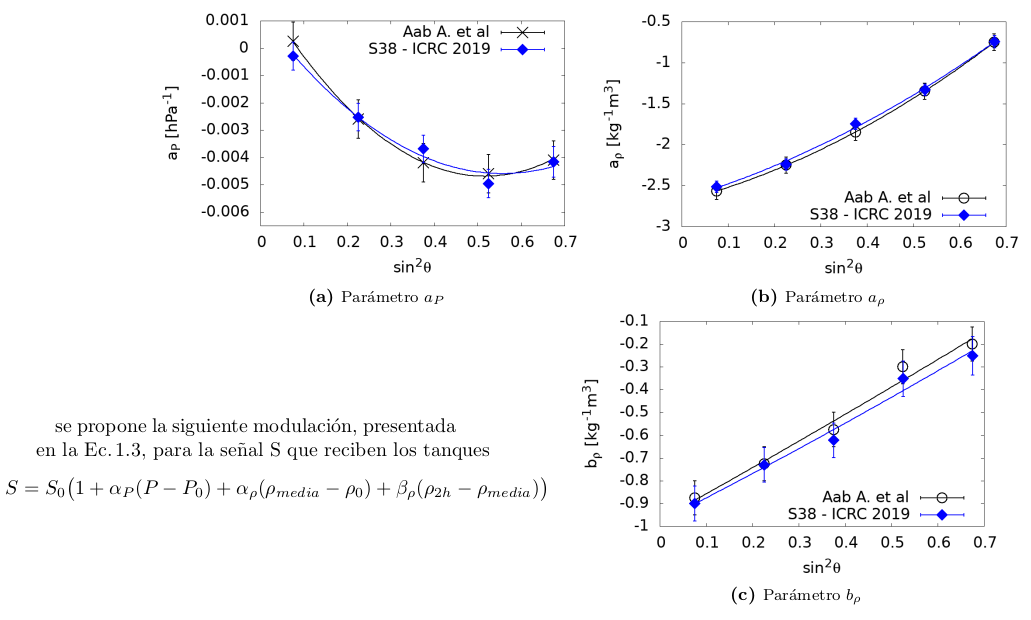
\includegraphics[width=0.95\textwidth]{../beamer-07-05-2020/tesis.png}
%   \end{figure}
  
% \section{Acerca del archivo con todos los disparos}

%   \begin{itemize}
%   	\item Diferencias con el disparo tradicional.
%     \begin{itemize}
%       \item[-] Empieza en el 2013
%       \item[-] Eficiencia
%       \item[-] Cantidad de datos en el bin de 1 EeV - 2 EeV.
%     \end{itemize}
%   	\item Pesos de los hexágonos.
%   	\item Resultados con el rango de energía 1 EeV - 2 EeV.
%     \item ¿Podemos mejorarlo con la corrección del clima?
%   \end{itemize}

\section{Cálculo de Rayleigh para el análisis de anisotropía}

  \subsubsection{Pesos de los hexágonos} \label{peso_hexagonos}

      % \begin{enumerate}
      %   \item Fijo una frecuencia a estudiar.
      %   \item Me muevo en el dataset de hexagonos, a cada utc lo clasifico según:
      %   \begin{equation*}
      %     h = (\text{hora local })\times \nicefrac{\text{Frecuencia a estudiar}}{\text{Frecuencia Solar}}
      %   \end{equation*}
      %     \item El valor de h no es continuo, sino está divido en 288 segmentos entre 1 y 24
      %  \item Le asigno un peso al bin h:
      %   \begin{align*}
      %     \text{peso del bin h} &= \nicefrac{\text{Hexagonos que cayeron en el bin h}}{I}\\
      %     I &= \sum^{288}_h \nicefrac{\text{Hexagonos que cayeron en el bin h}}{288}
      %    \end{align*} 
      % \end{enumerate}

      \begin{enumerate}
        \item Fijo un periodo a estudiar $T$
        \item Tomando en cuenta el registro de la cantidad de hexágonos 6T5, cada dato se clasifica según la hora local multiplicado por un factor de fase
        \begin{equation*}
          h = (\text{hora local})\times \frac{T}{T_{Solar}}
        \end{equation*}
        donde $T_{Solar}$ el periodo asociado a la frecuencia solar, que equivale a $\sim 365.25$  días solares. %El factor $ \nicefrac{T}{T_{Solar}}$ tiene en cuenta una fase global sobre
        \item Para simplicar el cálculo del peso de los hexágonos, se divide las 24 horas del día en $288$ segmentos de 5 min cada uno. Dado que el factor $\nicefrac{T}{T_{Solar}}$ podría ser mayor que 1, se toma $h' = h\, mod \,24$ \footnote{mod representa la función módulo.} para posteriormente asignar al segmento correspondiente. Por ejemplo, $h=25.0$ implica que $h'= 1.0$, que corresponde al doceavo segmento de $5$ min de un día.

       \item A medida que voy a asignando los hexágonos 6T5 a cada segmento, voy sumando la cantidad de 6T5. Para definir el peso que tiene un segmento $k$ en particular, primero calculo la media de hexágonos por segmento:
       \begin{equation}
         I = \sum^{288}_i \frac{\text{Hexágonos que cayeron en el segmento  i }}{288} = \sum^{288}_{i=1} \frac{N_{hex, i}}{288}
       \end{equation}
       Una vez obtenido este valor, podemos calcular el peso de segmento $k$  $w_{k,hex}$  como
        \begin{align}
         w_{k,hex}= \frac{N_{hex, k}}{I}
         \end{align} 
      \end{enumerate}

      Un ejemplo de lo que se obtiene


        \begin{figure}[H]
          \centering
              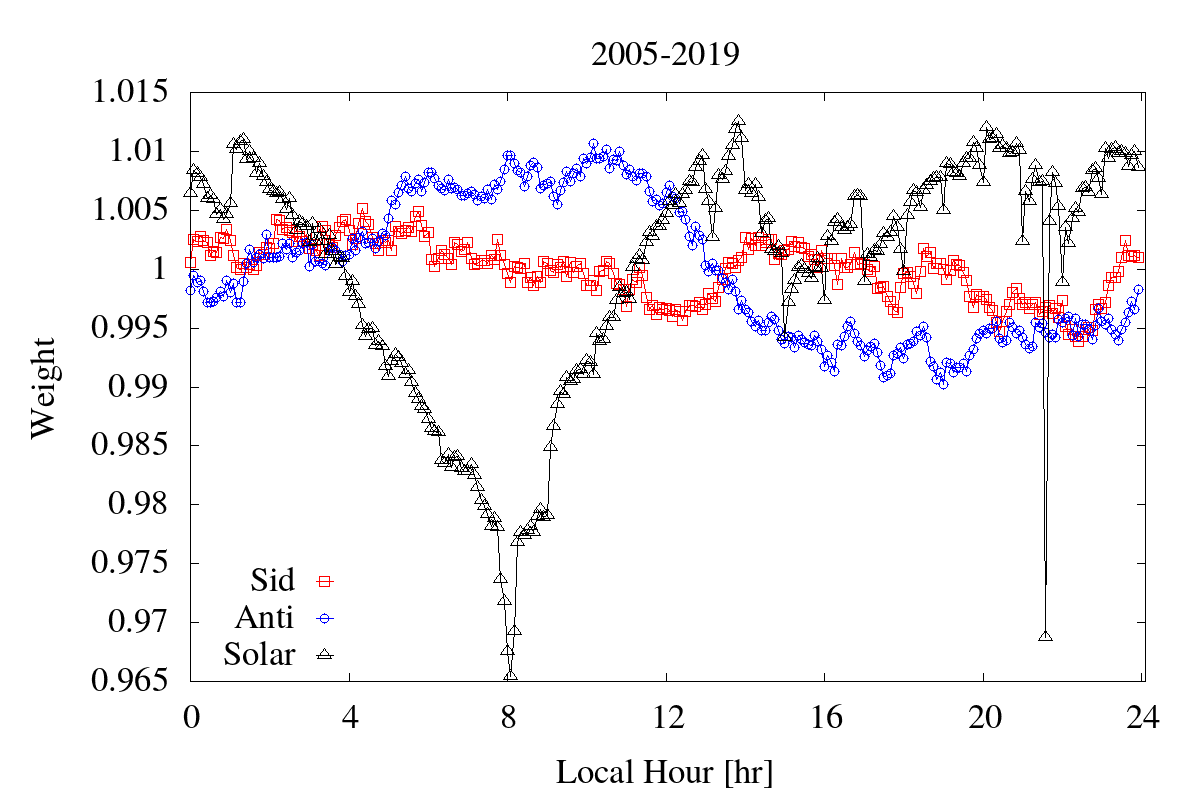
\includegraphics[width=0.85\linewidth]{../report_2_27_04_2020/Graficos/weigth2005-2019.png}
              \caption{Pesos de los hexágonos en el rango 2005-2019 para distintas frecuencias.}
        \end{figure}

  \subsubsection{Cálculo de Rayleigh para una frecuencia dada}

      % \begin{enumerate}
      %   \item Fijo una frecuencia a estudiar.
      %   \item Me muevo en el cielo con esa frecuencia (fase).
      %   \item Dado el utc del evento, lo clasifico según:
      %   \begin{equation*}
      %     h = (\text{hora local })\times \nicefrac{\text{Frecuencia a estudiar}}{\text{Frecuencia Solar}}
      %   \end{equation*}
      %     \item El valor de h no es continuo, sino está divido en 288 segmentos entre 1 y 24
      %  \item Le asigno un peso por evento:
      %   \begin{equation*}
      %     \text{peso del evento} = (\text{peso  de los hexágonos para el bin h})^{-1}
      %     \end{equation*} 
      %    \item Hago el análisis en frecuencias:
      %    \begin{align*}
      %        a &= \sum^{Eventos}_i \cos(2\pi \nicefrac{h}{24} + (RA -RA_{cenit}))\times \nicefrac{(\text{peso del evento})_i}{N}\\
      %        b &= \text{Lo mismo pero con seno}\qquad         N = \sum^{Eventos}_i \text{peso del evento}_i
      %    \end{align*}
      % \end{enumerate}

            \begin{enumerate}
        \item Fijando un rango de tiempo, estudiamos una frecuencia en particular, para el cálculo consideramos el periodo $T$
        \item Con los eventos ya filtrados, clasifico cada evento $i$ según la hora local por un fase
        \begin{equation*}
          h = (\text{hora local del evento } i)\times \frac{T}{T_{Solar}}
        \end{equation*}
        \item Este paso es parecido al paso $3$ del peso de los hexágonos donde obtengo $h'$ a partir de $h$. A diferencia que en este proceso, no es importante la cantidad de hexágonos, sino los pesos asignados a cada segmento en  la sección \ref{peso_hexagonos}. Una vez que le asigno un segmento $k$ a un evento $i$, el mismo pasa a tener un peso dado por:
        \begin{equation*}
          \text{peso del evento } i = w_{i}= (w_{k, hex})^{-1}
          \end{equation*} 
         
        \item Para el análisis en frecuencias, se necesita calcular los coeficientes de Fourier del primer armónico $a$ y $b$, para este caso se calculan de la siguiente manera:

        \begin{enumerate}
          \item Por cada evento se calculan los siguientes valores:
          \begin{align}
             a_i' &= {w_i}\cos\Big(2\pi \frac{h'}{24} + RA_i -RA_{cenit,i}\Big)\\
             b_i' &= {w_i}\sin\Big(2\pi \frac{h'}{24} + RA_i -RA_{cenit,i}\Big)\\
         \end{align}
         
         \item Una vez que se obtuvieron los valores de $a_i'$ y $b_i'$ para todos los eventos en el rango de tiempo estudiado, se calculan los coeficientes mediante:
         \begin{alignat}{1}
          \mathcal{N} &= \sum^{Eventos}_i w_i\\ 
            a &= \frac{2}{\mathcal{N}} \sum^{Eventos}_i a_i' \qquad
            b = \frac{2}{\mathcal{N}} \sum^{Eventos}_i b_i'  
         \end{alignat}
        \end{enumerate}

        \item Con los coeficientes es posible calcular la amplitud de la frecuencia estudiada $\tilde{r}$ y la fase $\phi$. Otros parámetros calculados para el análisis son la probabilidad $P(\tilde{r})$ de que la amplitud obtenida sea producto de una variación de ruido, y el valor de amplitud $r_{99}$ para que dicha probabilidad sea del $1$\%. 
        \begin{alignat}{3}
            \tilde{r} &= \sqrt{a^2 +b^2}             
            &&\phi&&= \arctan\frac{a}{b}\\
            P(\tilde{r})&= \exp(-\mathcal{N}\frac{\tilde{r}^2}{4}) \qquad
            &&r_{99}&&= \sqrt{\frac{-4\log(0.01)}{\mathcal{N}}}
        \end{alignat}



      \end{enumerate}